\documentclass[12pt]{article}
\usepackage{tikz}
\usetikzlibrary{shapes.geometric,arrows.meta,positioning,calc}
\usepackage{geometry}
\geometry{a4paper,margin=2.5cm}

\definecolor{stepblue}{RGB}{220,232,245}
\definecolor{stepborder}{RGB}{70,110,160}
\definecolor{periodbg}{RGB}{240,240,240}
\definecolor{periodborder}{RGB}{120,120,120}

\begin{document}
\begin{figure}[htbp]
\centering
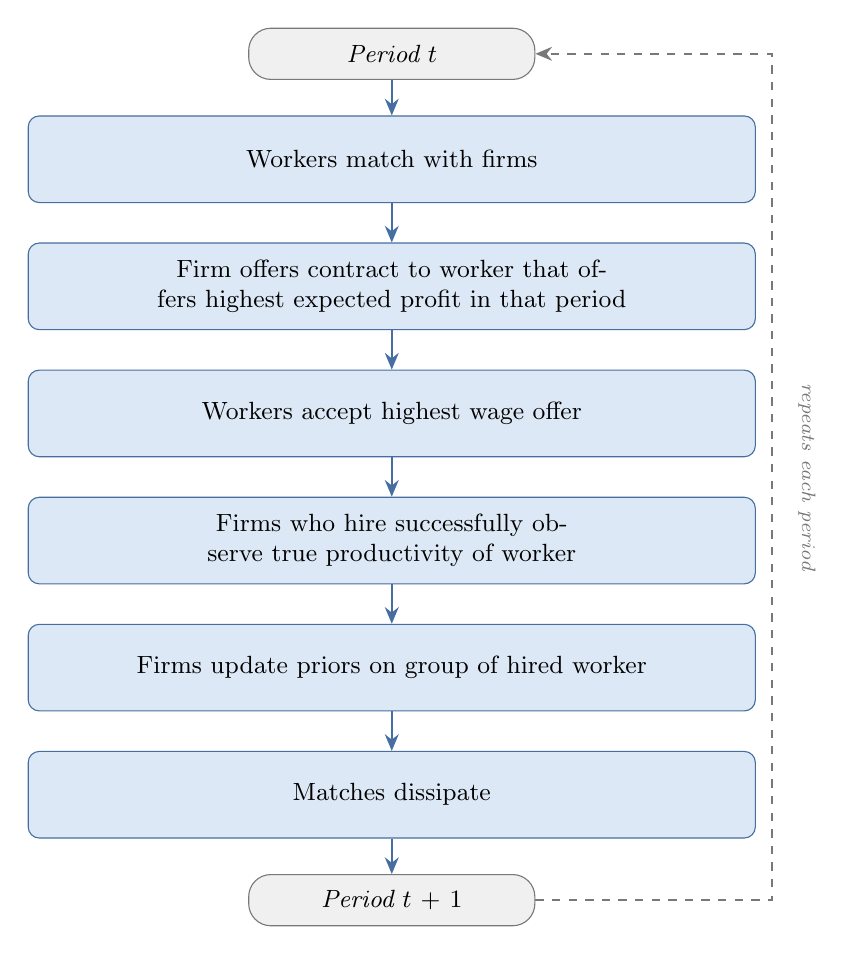
\begin{tikzpicture}[
  stagebox/.style={rectangle,rounded corners=4pt,draw=stepborder,fill=stepblue,
                   text width=9cm,minimum height=1.1cm,align=center,font=\small},
  periodbox/.style={rectangle,rounded corners=8pt,draw=periodborder,fill=periodbg,
                    text width=3.4cm,minimum height=0.65cm,align=center,font=\small\itshape},
  arr/.style={-{Stealth[length=6pt,width=5pt]},line width=0.8pt,color=stepborder},
  looparr/.style={-{Stealth[length=6pt,width=5pt]},line width=0.7pt,color=periodborder,dashed},
  node distance=0.5cm
]

\node[periodbox] (P1) {Period $t$};
\node[stagebox, below=0.45cm of P1] (S1)
    {Workers match with firms};
\node[stagebox, below=0.5cm of S1] (S2)
    {Firm offers contract to worker that offers highest expected profit in that period};
\node[stagebox, below=0.5cm of S2] (S3)
    {Workers accept highest wage offer};
\node[stagebox, below=0.5cm of S3] (S4)
    {Firms who hire successfully observe true productivity of worker};
\node[stagebox, below=0.5cm of S4] (S5)
    {Firms update priors on group of hired worker};
\node[stagebox, below=0.5cm of S5] (S6)
    {Matches dissipate};
\node[periodbox, below=0.45cm of S6] (P2) {Period $t+1$};

\draw[arr] (P1.south) -- (S1.north);
\draw[arr] (S1.south) -- (S2.north);
\draw[arr] (S2.south) -- (S3.north);
\draw[arr] (S3.south) -- (S4.north);
\draw[arr] (S4.south) -- (S5.north);
\draw[arr] (S5.south) -- (S6.north);
\draw[arr] (S6.south) -- (P2.north);

% Loop arrow: fixed x-offset of 3cm from box east edges
\coordinate (loopA) at ($(P2.east)+(3.0,0)$);
\coordinate (loopB) at ($(P1.east)+(3.0,0)$);
\draw[looparr] (P2.east) -- (loopA) -- (loopB) -- (P1.east);

% Label on the vertical segment, 0.45cm right of the dashed line
\node[font=\scriptsize\itshape,color=periodborder,rotate=-90,anchor=center]
  at ($(loopA)!0.5!(loopB)+(0.45,0)$) {repeats each period};

\end{tikzpicture}
\caption{Timeline of the model. Each period $t$ consists of six sequential
         stages; at the close of period $t$ the cycle repeats for period $t+1$.}
\label{fig:timeline}
\end{figure}
\end{document}
